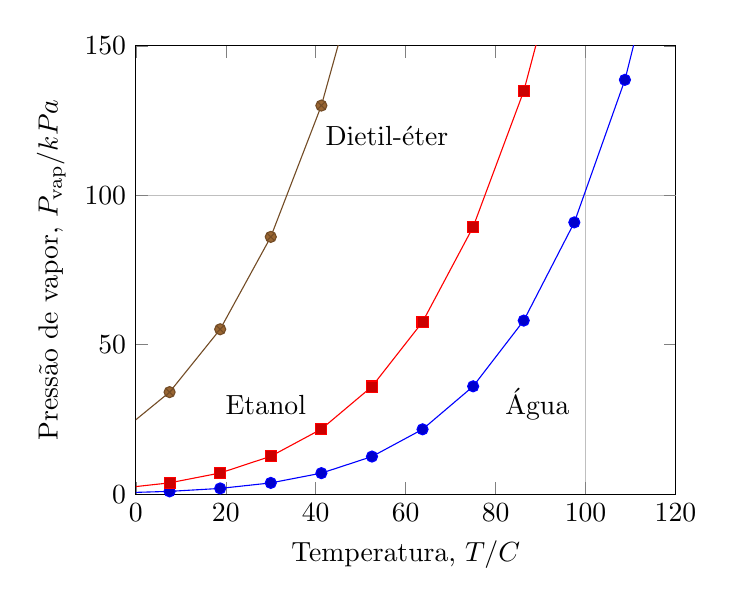
\begin{tikzpicture}
\begin{axis}
        [
            grid = minor,
            ylabel = {Pressão de vapor, $P_\mathrm{vap}/\unit{kPa}$},
            xlabel = {Temperatura, $T/\unit{\degree C}$},
            xmin = 0, xmax = 120,
            ymin = 0, ymax = 150,
            extra y ticks = {100},
            extra y tick labels = {},
            extra y tick style = { grid = major },
            extra x ticks = {100},
            extra x tick labels = {},
            extra x tick style = { grid = major },
        ]     
        % %%% BENZENO
        %  \addplot+ [domain = -150:120]
        %      { 
        %         100 * exp(-31*1000/8.3 * (1/(273 + x) - 1/(354)))
        %      };
        %%% AGUA
        \addplot+ [domain = -150:120]
            { 
                100 * exp(-44*1000/8.3 * (1/(273 + x) - 1/(373)))
            };
        \node [anchor = west] at      (axis cs:80,30) 
            {Água};
        %%% ETANOL
        \addplot+ [domain = -150:120]
            { 
                100 * exp(-38*1000/8.3 * (1/(273 + x) - 1/(351)))
            };
        \node [anchor = east] at      (axis cs:40,30) 
            {Etanol};
        %%% DIETIL ÉTER
        \addplot+ [domain = -150:120]
            { 
                100 * exp(-29*1000/8.3 * (1/(273 + x) - 1/(307)))
            };
        \node [anchor = west] at      (axis cs:40,120) 
            {Dietil-éter};
\end{axis}
\end{tikzpicture}